\documentclass{article}


\usepackage{arxiv}

\usepackage[utf8]{inputenc} % allow utf-8 input
\usepackage[T1]{fontenc}    % use 8-bit T1 fonts
\usepackage{hyperref}       % hyperlinks
\usepackage{url}            % simple URL typesetting
\usepackage{booktabs}       % professional-quality tables
\usepackage{amsfonts}       % blackboard math symbols
\usepackage{nicefrac}       % compact symbols for 1/2, etc.
\usepackage{microtype}      % microtypography
\usepackage{lipsum}
\usepackage[ruled,vlined]{algorithm2e}

\title{A template for the \emph{arxiv} style}


% \author{Gilad Ben Or\\% Name author
%     \href{mailto:benorgi@post.bgu.ac.il}{\texttt{benorgi@post.bgu.ac.il}} %% Email author 1 
% % }

\author{
  Gilad Ben Or\\
  ID: 036256527\\
  \texttt{benorgi@post.bgu.ac.il} \\
  }
%   %% examples of more authors
%   \And
%  Elias D.~Striatum \\
%   Department of Electrical Engineering\\
%   Mount-Sheikh University\\
%   Santa Narimana, Levand \\
%   \texttt{stariate@ee.mount-sheikh.edu} \\
%   %% \AND
% %   %% Coauthor \\
%   %% Affiliation \\
%   %% Address \\
%   %% \texttt{email} \\
%   %% \And
%   %% Coauthor \\
%   %% Affiliation \\
%   %% Address \\
%   %% \texttt{email} \\
%   %% \And
%   %% Coauthor \\
%   %% Affiliation \\
%   %% Address \\
%   %% \texttt{email} \\
% }

\begin{document}
\maketitle

\begin{abstract}
\lipsum[1]
\end{abstract}


% keywords can be removed
\keywords{First keyword \and Second keyword \and More}


% --------------------
\section{Introduction}
% --------------------
Many high-performance machine learning algorithms are susceptible to minimal changes in their inputs. Adversarial perturbations drawn attention from two directions. On the one hand, we are concerned about the integrity and security of machine learning algorithms deployed, such as autonomous cars or face-recognition systems. On the other hand, it is a exciting research opportunity to understand the difference between human and computer sensory information processing.

Decision-based attacks are a category of black box attacks which depend solely on the model's final decision. In terms of the structure of the inputs and outputs and certain examples classified by the model, the attacker has little knowledge regarding the  the model to be attacked.

Previous works suggested algorithms for finding adversarial examples with minimal perturbation size and minimal calls of the model to be attacked. \cite{brendel2017decision} introduced a the boundary attack that starts from a large adversarial perturbation and then seeks to reduce the perturbation while staying adversarial. \cite{chen2019hopskipjumpattack} proposed a novel unbiased estimate of gradient direction at the decision boundary based solely on access to model decisions. Their algorithms requires significantly fewer model queries than several state-of-the-art decision-based adversarial attacks and achieves competitive performance in attacking several widely-used defense mechanisms.

In order to design and evaluate more attack algorithms, there is a real need for an environment that allows data interaction and results measurement. An existing, well known and powerful environment is CleverHans. CleverHans \cite{papernot2018cleverhans} is a software library that provides standardized reference implementations of adversarial example construction techniques and adversarial training. The library may be used to develop more robust machine learning models and to provide standardized benchmarks of models' performance in the adversarial setting. 

I looked at the same problems that CleverHans encountered and sought to address in a different way. I have observed that the requirements of the testing environment are similar and may be reduced to those of the reinforcement learning environment.
Reinforcement learning environment offers the opportunity to observe data , perform a single or sequence of actions and receive the corresponding score. Here, the attack algorithms are equivalent to the reinforcement learning policies.

The use of such an environment will improve the implementation of new algorithms and will be a standard tool for testing them. Thus, researchers may be able to work with state-of-the-art algorithms and methodologies, reinforcement learning in particular.

In this work, I developed a decision-based attack environment based on the OpenAI Reinforcement Learning Gym \cite{brockman2016openai} interface. The system fits for the MNIST dataset \cite{mnist10027939599} and can quickly be expanded to support other datasets. I have researched and added support for custom actions, implemented two policies and trained a reinforcement learning agent to discover the optimal policy.

The contributions of this work are as follows:
\begin{itemize}
\item Introduce a research framework for decision-based attacks. 
\item Suggests custom actions for attack algorithms.
\item Design, implementation and evaluation of two boundary attack algorithms.
\item Training and evaluation of reinforcement learning agent in this environment.
\end{itemize}

% --------------------
\section{Research Question}
% --------------------

The question or gap you were trying to answer as part of this research

% --------------------
\section{Hypothesis}
% --------------------
Your initial hypothesis or assumption when addressing the research question

% --------------------
\section{Material and methods}
% --------------------

\subsection{Data}
I used the MNIST \cite{mnist10027939599} dataset for this work. The dataset was downloaded using Keras API without any additional prepossessing. 
The MNIST dataset has a training set of 60,000 examples, and a test set of 10,000 examples. It is a subset of a larger set available from NIST. The original black and white (bilevel) images from NIST were size normalized to fit in a 20x20 pixel box while preserving their aspect ratio. The resulting images contain grey levels as a result of the anti-aliasing technique used by the normalization algorithm. the images were centered in a 28x28 image by computing the center of mass of the pixels, and translating the image so as to position this point at the center of the 28x28 field. \\

\subsection{The model to be attacked}
The model I would like to attacked is the convolution neural network used during the course labs. It achieved accuracy performance of 0.975.

\subsection{Evaluation environment}
I chose OpenAI Gym \cite{brockman2016openai} as my evaluation environment. Gym is a toolkit for developing and comparing reinforcement learning algorithms. It makes no assumptions about the structure of the tested agent, and is compatible with any numerical computation library, such as TensorFlow or Theano.
I selected this environment as it enables various algorithms to be fitted and tested. In specific, it is appropriate for both the deterministic method and the reinforcement learning algorithm. \\
In order to register a new environment, I implemented the following 4 methods: constructor, reset, render and step.
\subsubsection{Constructor}
In the environment's constructor I loaded the dataset, initiated the MNIST classifier (the model to be attacked) and checked that it perform well.

\subsubsection{Reset}
This method resets the environment to initial state and return first observation (see below).
Here, it does the following things:
\begin{enumerate}
\item Choose a benign example (from the training or the testing sets, depending on the environment mode).
\item Generate two centers (see below).
\item Reset initial variables such as the initial step size, max perturbation and etc.
\end{enumerate}

\subsubsection{Step}
This method commits an action a and return a new observation,  a reward, the is done signal and additional info (all explained below).

\subsubsection{Observation}
The observation is an environment-specific object representing the agent's observation of the environment. The observation consists of the following objects:
\begin{enumerate}
\item \textbf{current image} - the image of the current step.
\item \textbf{classifier prediction} - the classifier's prediction for the current image.
\item \textbf{perturbation norm} - the perturbation norm of the current image with respect to the source image.
\item \textbf{steps} - the index of the current step.
\end{enumerate}

\subsubsection{Action space}
The following actions are available for the agent:
\begin{enumerate}
\item 
\textbf{Decrease step} - 
Decrease the step size according to the equation below.: \\
step=\begin{Bmatrix}
step size > 0.4 : step size/2\\ 
o.w.: max(0.05, step_size- 0.05)
\end{Bmatrix}
\item 
\textbf{Increase step} - 
Increase the step size according to the equation below.: \\
step=\begin{Bmatrix}
step size > 0.4 : step size/2\\ 
o.w.: max(0.05, step_size- 0.05)
\end{Bmatrix}

\item 
\textbf{Closet cluster} - 
Go one step in the direction of the nearest target cluster.

\item 
\textbf{Farthest cluster} - 
Go one step in the direction of the most distant target cluster.

\item 
\textbf{Original image} - 
Go one step in the direction of the original sample.

\item 
\textbf{New centers} - 
Generate new centers. In offline, the environment randomly generates 20 samples with the target label and select a pair of samples with the largest distance between them. The output of this process is 2 target samples which called centers. The agent calculates the distance to each center at each step. The closest target center called "closest cluster" and farthest one called "farthest center".
\end{enumerate}

\subsubsection{Reward}
The reward has to take into account two factors:
\begin{enumerate}
\item The classification of the adversarial example - whether the classifier labeles the examples as the target class.
C=\begin{Bmatrix}
1: x\in targetclass\\ 
0: x\notin targetclass
\end{Bmatrix}
\item Perturbation size - the agent gets negative reward if the perturbation is bigger than maximum perturbation P and positive reward if it under this limit.
\end{enumerate}

A suggestion for the reward function is shown in (Equation \ref{eq1}):
\begin{equation} \label{eq1}
reward = \alpha C + \beta  \left (P-d\left ( o, t \right )  \right )
\end{equation}

\subsubsection{Is done signal}
The is done signal stops the agent while it does the exploration-exploitation tasks. We would stop the agent if it perform more than L steps, or it reached the target class under the perturbation size constraint.

\subsection{Deterministic agents}
In this section I describe two deterministic agents that were evaluated in the this work. The agents' policy was described using a graph. The agents moves from initial state and takes an action based on the current state and observation.


\subsubsection{The triangle agent}
The triangle agent used a policy as described in \ref{alg: simple}. It used one source point and two target points to explore the boundary and then to move in a triangle track from point to point in order to reduce the perturbation. In each cycle, the agent decreases the step size.

\begin{algorithm}[H] \label{alg:simple}
\SetAlgoLined
\KwResult{Adversarial image}
 initialization\;
 \While{perturbation \geq PERTURBATION SIZE, steps \leq MAX STEPS }{
 go in the direction of the closet center until labeled as target;\\
 decrease step size;\\
 go in the direction of the source sample until labeled as source;\\
 (option) decrease step size;\\
 go in the direction of the farthest center until labeled as target;\\
 (option) decrease step size;\\
 go in the direction of the source sample until labeled as source;\\
 (option) decrease step size;\\
 }
 \caption{Simple agent}
\end{algorithm}

\subsubsection{The alternating triangle agent}
The alternating triangle agent is an enhancement of the triangle agent. It executes the triangle agent for K steps, takes the best observation and used it as the initial step for the next agent. It may keep the current step size or increase it back to the initial step size.

to  used a policy as described in \ref{alg: simple}. It used one source point and two target points to explore the boundary and then to move in a triangle track from point to point in order to reduce the perturbation. In each cycle, the agent decreases the step size.

\begin{algorithm}[H] \label{alg:simple}
\SetAlgoLined
\KwResult{Adversarial image}
 initialization\;
 \While{perturbation \geq PERTURBATION SIZE, steps \leq MAX STEPS }{
 go in the direction of the closet center until labeled as target;\\
 decrease step size;\\
 go in the direction of the source sample until labeled as source;\\
 (option) decrease step size;\\
 go in the direction of the farthest center until labeled as target;\\
 (option) decrease step size;\\
 go in the direction of the source sample until labeled as source;\\
 (option) decrease step size;\\
 }
 \caption{Simple agent}
\end{algorithm}





\subsection{Reinforcement learning model}
The purpose of reinforcement learning model is to teach an agent to take actions in an environment in order to maximize the cumulative reward. In this work, the agent learns how to take actions in order to generate an adversarial example for a target class while maximize the rewards which is relative to its success in generating an adversarial example with minimal perturbation size.

Figure \ref{fig:rl_model} shows a widely used reinforcement learning framework. The agent accesses the environment, triggers it with an action, collects the reward and observes the new state of the environment.

In the following subsections we describe each component in the figure.

\begin{figure}[H]
    \centering
        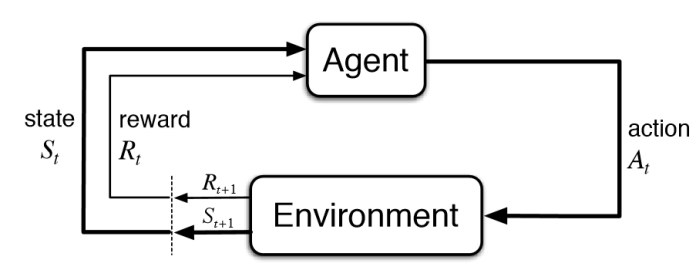
\includegraphics[scale=.8]{figures/reinforcement-learning-fig1-700.jpg}
    \caption{Reinforcement learning framework.}
    \label{fig:rl_model}
\end{figure}

\textbf{Note:} We will have to train a different agent for each target label. \\




\subsection{The agent}
The agent will learn his policy using one of the common reinforcement learning methods such as SARSA, DQN and etc.

\subsection{Evaluation}
\subsubsection{dataset}
MNIST

\subsubsection{The attacked classifier}
Black box convolution network based classifier.

\subsubsection{metrics}
We will measure the number of classifier calls for a generation of an adversarial example.

systemitic vs randomizsation

Because in the final layer you are approximating a real state action value for each action. You output to a linear layer as your Q value estimate can generally take on any real value. And then you add a mean squares error loss with the linear layer output.

This set up is similar any general regression problem with a neural nnetwork.

Relu is used quite often but for hidden layer activation.

Softmax output is quite popular for representing the policy network/function for discrete actions. But for Q learning, we are learning an approximate estimate of the Q value for each state action pair, which is a regression problem.

    # Select a policy. We use eps-greedy action selection, which means that a random action is selected with probability eps. We anneal eps from 1.0 to 0.1 over the course of 1M steps. This is done so that the agent initially explores the environment (high eps) and then gradually sticks to what it knows (low eps). We also set a dedicated eps value that is used during testing. Note that we set it to 0.05 so that the agent still performs some random actions. This ensures that the agent cannot get stuck.



Hyperparam
Transferability 
Many calls
Dataset 
Yaron

\subsection{Agents}
In this section we described the agents that I design and tested in this work. The first two agents are unique to this work, and the last one is a common reinforcement learning agent.

% --------------------
\section{Results}
% --------------------

\begin{table}[]
\caption{Simple centers algorithm. The table explains the details about the minimal perturbations that happened in the episodes. Min perturbations is the minimum perturbations reached in all episodes. Max perturbations is the maximum perturbations over all the episodes' perturbation.}
\label{tab:simple_result}
\begin{tabular}{|l|l|l|l|l|l|l|l|l|l|}
\hline
\textbf{}       & \textbf{}     & \multicolumn{4}{c|}{\textbf{perturbation}}                      & \multicolumn{4}{c|}{\textbf{steps}}                             \\ \hline
\textbf{target} & \textbf{nobs} & \textbf{min} & \textbf{max} & \textbf{mean} & \textbf{variance} & \textbf{min} & \textbf{max} & \textbf{mean} & \textbf{variance} \\ \hline
0 & 100  & 3.79     & 7.84     & 5.42      & 0.97          & 2         & 1895      & 194.2      & 168529.84      \\ \hline
1 & 100  & 2.0      & 11.33    & 6.23      & 2.37          & 1         & 1273      & 44.42      & 20352.17       \\ \hline
2 & 100  & 2.0      & 9.01     & 5.35      & 1.89          & 1         & 1994      & 191.41     & 216859.19      \\ \hline
3 & 100  & 3.59     & 10.72    & 5.79      & 1.81          & 2         & 1978      & 188.25     & 190226.86      \\ \hline
4 & 100  & 3.55     & 10.04    & 5.78      & 1.71          & 2         & 1632      & 160.87     & 150310.03      \\ \hline
5 & 100  & 3.07     & 9.6      & 6.2       & 1.84          & 2         & 401       & 19.24      & 2625.3         \\ \hline
6 & 100  & 2.0      & 10.24    & 5.87      & 2.01          & 1         & 1987      & 207.7      & 195911.51      \\ \hline
7 & 100  & 3.54     & 9.42     & 6.06      & 2.14          & 2         & 1979      & 192.28     & 211393.82      \\ \hline
8 & 100  & 2.0      & 10.3     & 5.28      & 1.62          & 1         & 1940      & 192.8      & 192080.91      \\ \hline
9 & 100  & 3.8      & 8.73     & 5.69      & 1.34          & 2         & 1930      & 77.56      & 74499.2        \\ \hline
\end{tabular}
\end{table}


for all targets, there is a source example that is very close to the boundary, thus, one or two steps are enough to produce an adversarial example.


\begin{table}[]
\caption{Iterative centers algorithm results}
\label{tab:iterative_result}
\begin{tabular}{|l|l|l|l|l|l|l|l|l|l|}
\hline
\textbf{}       & \textbf{}     & \multicolumn{4}{c|}{\textbf{perturbation}}                      & \multicolumn{4}{c|}{\textbf{steps}}                             \\ \hline
\textbf{target} & \textbf{nobs} & \textbf{min} & \textbf{max} & \textbf{mean} & \textbf{variance} & \textbf{min} & \textbf{max} & \textbf{mean} & \textbf{variance} \\ \hline
0 & 100  & 3.52     & 6.57     & 5.15      & 0.56          & 2         & 1998      & 1240.96    & 337448.91      \\ \hline
1 & 100  & 3.71     & 9.9      & 5.87      & 1.56          & 2         & 1924      & 840.9      & 413978.66      \\ \hline
2 & 100  & 2.0      & 7.26     & 5.02      & 0.86          & 1         & 1999      & 894.11     & 456457.01      \\ \hline
3 & 100  & 3.73     & 8.01     & 5.18      & 1.1           & 2         & 1993      & 1154.96    & 427066.36      \\ \hline
4 & 100  & 3.25     & 7.96     & 5.24      & 1.07          & 2         & 1994      & 1147.4     & 426411.49      \\ \hline
5 & 100  & 3.02     & 8.61     & 5.75      & 1.47          & 2         & 1810      & 240.7      & 131112.35      \\ \hline
6 & 100  & 2.0      & 8.34     & 5.38      & 0.96          & 1         & 1991      & 1391.65    & 250875.6       \\ \hline
7 & 100  & 3.52     & 8.02     & 5.41      & 1.28          & 2         & 1993      & 877.99     & 397813.36      \\ \hline
8 & 100  & 2.0      & 7.18     & 4.91      & 0.75          & 1         & 1940      & 1086.72    & 437924.24      \\ \hline
9 & 100  & 3.75     & 8.62     & 5.39      & 1.16          & 2         & 1989      & 1097.95    & 451468.78      \\ \hline
\end{tabular}
\end{table}


200000 - 2383(40min) - 0000 - DECREASE_STEP
200000 - 2383(40min) - 0000 - CLOSET CLUSTER

% \includemedia[width=0.6\linewidth,height=0.6\linewidth,activate=pageopen,
% passcontext,
% transparent,
% addresource=myclip.mp4,
% flashvars={source=myclip.mp4}
% ]{\includegraphics[width=0.6\linewidth]{penguins}}{VPlayer.swf}

\begin{frame}
\frametitle{Forward Kinematics}

\begin{center}
\includemedia[
    activate=onclick,
    width=0.75\textwidth
]{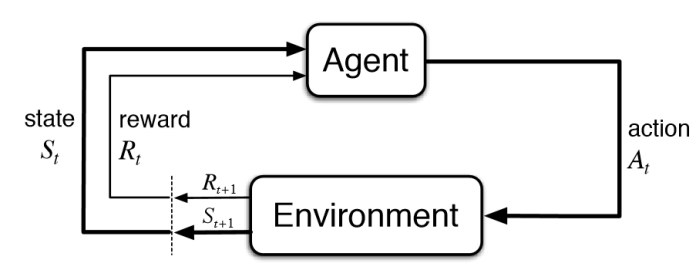
\includegraphics{figures/reinforcement-learning-fig1-700.jpg}}{myclip.mp4}
\end{center}
\end{frame}
Dummy text.

% --------------------
\section{Discussion and Conclusions}
% --------------------
Your interpretation of the results and findings
Dummy text. 


% --------------------
\section{Follow up steps}
% --------------------

Future work, things you wanted to accomplish but did not have the time to, open questions,

\bibliographystyle{apalike}  
\bibliography{references}  %%% Remove comment to use the external .bib file (using bibtex).
%%% and comment out the ``thebibliography'' section.


% %%% Comment out this section when you \bibliography{references} is enabled.
% \begin{thebibliography}{1}

% \bibitem{kour2014real}
% George Kour and Raid Saabne.
% \newblock Real-time segmentation of on-line handwritten arabic script.
% \newblock In {\em Frontiers in Handwriting Recognition (ICFHR), 2014 14th
%   International Conference on}, pages 417--422. IEEE, 2014.

% \bibitem{kour2014fast}
% George Kour and Raid Saabne.
% \newblock Fast classification of handwritten on-line arabic characters.
% \newblock In {\em Soft Computing and Pattern Recognition (SoCPaR), 2014 6th
%   International Conference of}, pages 312--318. IEEE, 2014.

% \bibitem{hadash2018estimate}
% Guy Hadash, Einat Kermany, Boaz Carmeli, Ofer Lavi, George Kour, and Alon
%   Jacovi.
% \newblock Estimate and replace: A novel approach to integrating deep neural
%   networks with existing applications.
% \newblock {\em arXiv preprint arXiv:1804.09028}, 2018.

% \end{thebibliography}


\end{document}
